\documentclass{exam}
\usepackage{graphicx}
\usepackage[utf8]{inputenc}
\usepackage[english]{babel}
\usepackage{amsmath}
\usepackage{hyperref}
\usepackage{amsthm}
\usepackage{tcolorbox}
\usepackage{amsfonts}
\usepackage{amssymb}
\usepackage{mathrsfs}
\usepackage{centernot}

\DeclareMathOperator{\lcm}{lcm}

\newcommand{\nimplies}{\centernot\implies}

\newbox\eeveebox
\setbox\eeveebox\hbox{
\raisebox{-2.5pt}{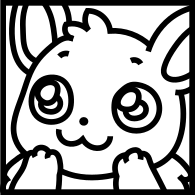
\includegraphics[height=2.5ex]{iibui.png}}}
\def\eeveeKawaii{\copy\eeveebox}

\newbox\skullbox
\setbox\skullbox\hbox{
\raisebox{-2.5pt}{
\includegraphics[height=2.5ex]{skull.png}}}
\def\bendingskull{\copy\skullbox}

\NewTColorBox{proposition}{m}{
  standard jigsaw,
  sharp corners,
  boxrule=0.4pt,
  coltitle=black,
  colframe=black,
  opacityback=0,
  opacitybacktitle=0,
  fonttitle=\normalfont\bfseries\upshape,
  fontupper=\normalfont\itshape,
  title={Proposition #1},
  after title={.},
  attach title to upper={\ },
}

\NewTColorBox{conjecture}{m}{
  standard jigsaw,
  sharp corners,
  boxrule=0.4pt,
  coltitle=black,
  colframe=black,
  opacityback=0,
  opacitybacktitle=0,
  fonttitle=\normalfont\bfseries\upshape,
  fontupper=\normalfont\itshape,
  title={Conjecture #1},
  after title={.},
  attach title to upper={\ },
}

\NewTColorBox{lemma}{m}{
  standard jigsaw,
  sharp corners,
  boxrule=0.4pt,
  coltitle=black,
  colframe=black,
  opacityback=0,
  opacitybacktitle=0,
  fonttitle=\normalfont\bfseries\upshape,
  fontupper=\normalfont\itshape,
  title={Lemma #1},
  after title={.},
  attach title to upper={\ },
}

\renewcommand\qedsymbol{$\eeveeKawaii$}

\title{Hammack Exercises - Chapter 9}
\author{FungusDesu}
\date{September 18th 2024}

\begin{document}

\maketitle

\section{Preface}
i dont really have anything to say

\section{Conjectures}

\begin{conjecture}{9.1}
    If $x, y\in\mathbb R$, then $\lvert x+y\rvert = \lvert x\rvert+\lvert y\rvert$.
\end{conjecture}

\begin{proof}[Disproof]
    This conjecture is false due to the following counterexample. Let $x=-69$ and $y=420$. Then $\lvert x+y\rvert=351$, whereas $\lvert x\rvert + \lvert y\rvert = 489$. Thus $\lvert x+y\rvert \neq \lvert x\rvert+\lvert y\rvert$.
\end{proof}

\begin{conjecture}{9.2}
    For every natural number $n$, the integer $2n^2-4n+31$ is prime.
\end{conjecture}

\begin{proof}[Disproof]
    This conjecture is false due to the following counterexample. Let $n = 31$. Then $2n^2-4n+31 = 1829 = 31\cdot59$. Thus $2n^2-4n+31$ is not prime.
\end{proof}

\begin{conjecture}{9.3}
    If $n\in\mathbb Z$ and $n^5-n$ is even, then $n$ is even.
\end{conjecture}

\begin{proof}[Disproof]
    This conjecture is false due to the following counterexample. Let $n=1$, which is odd. Then $n^5-n=0$, which is even. Thus $n^5-n$ is even, but $n$ itself is odd.
\end{proof}

\begin{conjecture}{9.4}
    For every natural number $n$, the integer $n^2+17n+17$.
\end{conjecture}

\begin{proof}[Disproof]
    This conjecture is false due to the following counterexample. Let $n = 17$. Then $n^2+17n+17 =595 =35\cdot17$. Thus $n^2+17n+17$ is not prime.
\end{proof}

\begin{conjecture}{9.5}
    If $A,B,C$ and $D$ are sets, then $(A\times B)\cup(C\times D)=(A\cup C)\times(B\cup D)$.
\end{conjecture}

\begin{proof}[Disproof]
    This conjecture is false due to the following counterexample. Let $A=\{1\},B=\{1, 2\}, C=\{3\}, D =\{2, 3\}$. Then $(A\times B)\cup(C\times D)=\{(1, 1), (1, 2), (3, 2), (3, 3)\}$, whereas $(A\cup C)\times(B\cup D) = \{(1, 1), (1, 2), (1, 3), (3, 1), (3, 2), (3, 3)\}$. Thus $(A\times B)\cup(C\times D)\neq(A\cup C)\times(B\cup D)$.
\end{proof}

\begin{conjecture}{9.6}
    If $A, B, C$ and $D$ are sets, then $(A\times B)\cap(C\times D)=(A\cap C)\times(B\cap D)$.
\end{conjecture}

This conjecture was proven earlier in the form of Lemma 8.1.

\begin{conjecture}{9.7}
    If $A, B$ and $C$ are sets, and $A\times C=B\times C$, then $A=B$.
\end{conjecture}

\begin{proof}[Disproof]
    This conjecture is false due to the following counter example. Let $A=\{1\}$, $B=\{2\}$ and $C=\varnothing$. Then $A\neq B$, but $A\times C=B\times C=\varnothing$. Thus $A\times C=B\times C$ does not imply $A=B$.
\end{proof}

\begin{conjecture}{9.8}
    If $A, B$ and $C$ are sets, then $A-(B\cup C)=(A-B)\cup(A-C)$.
\end{conjecture}

\begin{proof}[Disproof]
    This conjecture is false due to the following counterexample. Let $A = \{1\}$, $B= \{1, 2\}$, $C=\varnothing$. Note that $A-(B\cup C) = \varnothing$, whereas $(A-B)\cup(A-C) = \{1\}$. Thus $A-(B\cup C)\neq(A-B)\cup(A-C)$.
\end{proof}

\begin{conjecture}{9.9}
    If $A$ and $B$ are sets, then $\mathscr{P}(A)-\mathscr{P}(B)\subseteq\mathscr{P}(A-B)$.
\end{conjecture}

\begin{proof}[Disproof]
    This conjecture is false due to the following counterexample. Let $A =\{1, 2\}$ and $B=\{2\}$. Note that $\mathscr{P}(A) - \mathscr{P}(B) = \{\{1\}, \{1, 2\}\}$, whereas $\mathscr{P}(A-B)=\{\varnothing, \{1\}\}$. Thus $\mathscr{P}(A)-\mathscr{P}(B)\nsubseteq\mathscr{P}(A-B)$.
\end{proof}

\begin{conjecture}{9.10}
    If $A$ and $B$ are sets and $A\cap B=\varnothing$, then $\mathscr{P}(A)-\mathscr{P}(B)\subseteq\mathscr{P}(A-B)$.
\end{conjecture}

This conjecture is true. To prove it, we shall suppose $A\cap B=\varnothing$ for arbitrary sets $A$ and $B$, and show that $\mathscr{P}(A)-\mathscr{P}(B)\subseteq\mathscr{P}(A-B)$. A proof follows.
\begin{proof}
    Suppose $A\cap B = \varnothing$; then there does not exist $x$ such that $x\in A\land x\in B$. We have the following:
    \begin{align*}
        A-B=\{x:x\in A\land x\notin B\} = A.
    \end{align*}
    Thus $\mathscr{P}(A)-\mathscr{P}(B)\subseteq\mathscr{P}(A)=\mathscr{P}(A-B)$.
\end{proof}

\begin{conjecture}{9.11}
    If $a,b\in\mathbb N$, then $a+b<ab$.
\end{conjecture}

\begin{proof}[Disproof]
    This conjecture is false due to the following counterexample. Let $a = b = 1$. Note that $a + b = 2$, whereas $ab = 1$. Thus $a+b>ab$.
\end{proof}

\begin{conjecture}{9.12}
    If $a, b, c\in\mathbb N$ and $ab$, $bc$ and $ac$ all have the same parity, then $a,b$ and $c$ all have the same parity.
\end{conjecture}

\begin{proof}[Disproof]
    This conjecture is false due to the following counterexample. Let $a = 2$, $b=3$ and $c = 4$. Note that $ab = 6$, $bc = 12$ and $ac = 8$; and so $ab$, $bc$ and $ac$ have the same parity while $a$, $b$ and $c$ themselves do not.
\end{proof}

\begin{conjecture}{9.13}
    There exists a set $X$ for which $\mathbb R\subseteq X$ and $\varnothing\in X$.
\end{conjecture}

This conjecture is true. We shall provide an example set $X$ for which $\mathbb R\subseteq X$ and $\varnothing\in X$. A proof follows.
\begin{proof}
    Consider $X = \mathbb R\cup\{\varnothing\}$. Note that $R\subseteq X$ and $\varnothing\in X$. We have found a set $X$ that satisfies such properties.
\end{proof}

\begin{conjecture}{9.14}
    If $A$ and $B$ are sets, then $\mathscr P(A)\cap\mathscr P(B)=\mathscr P(A\cap B)$.
\end{conjecture}

This conjecture is true. To prove this, we shall show that $\mathscr P(A)\cap\mathscr P(B)\subseteq\mathscr P(A\cap B)$ and vice versa. A proof follows.

\begin{proof}
    $(\subseteq)$ Suppose $X\in\mathscr P(A)\cap\mathscr P(B)$. Then $X\subseteq A$ and $X\subseteq B$. Let $x\in X$; since $x\in A$ and $x\in B$, we have $x\in A\cap B$. This implies $X\subseteq A\cap B$, and so $X\in\mathscr P(A\cap B)$.

    $(\supseteq)$ Suppose $X\in\mathscr P(A\cap B)$. Then $X\subseteq A\cap B$. Let $x\in X$; since $x\in A\cap B$, we have $x\in A$ and $x\in B$. This implies $X\subseteq A$ and $X\subseteq B$, and so $X\in\mathscr P(A)\cap\mathscr P(B)$. This completes our proof.
\end{proof}

\begin{conjecture}{9.15}
    Every odd integer is the sum of three odd integers.
\end{conjecture}

This conjecture is true. A proof follows.

\begin{proof}
    Let $a, b, c\in\mathbb Z$ be odd. Then there exist $x,y,z\in\mathbb Z$ such that $a = 2x + 1$, $b=2y+1$, $c=2z + 1$. Thus we have the following:
    \begin{align*}
        a + b + c = 2x + 2y + 2z + 3 = 2(x + y + z + 1) + 1.
    \end{align*}
    This completes our proof.
\end{proof}

\begin{conjecture}{9.16}
    If $A$ and $B$ are finite sets, then $\lvert A\cup B\rvert=\lvert A\rvert +\lvert B\rvert$.
\end{conjecture}

\begin{proof}[Disproof]
    This conjecture is false due to the following counterexample. Let $A=\{1\}$ and $B=\{1,2\}$. Note that $\lvert A\cup B\rvert=2$, whereas $\lvert A\rvert+\lvert B\rvert=3$. Thus $\lvert A\cup B\rvert\neq\lvert A\rvert +\lvert B\rvert$.
\end{proof}

\begin{conjecture}{9.17}
    For all sets $A$ and $B$, if $A-B=\varnothing$, then $B\neq\varnothing$.
\end{conjecture}

\begin{proof}[Disproof]
    This conjecture is false due to the following counterexample. Let $A = B = \varnothing$. Note that $A - B = \varnothing$. Thus $A-B =\varnothing$ does not imply $B \neq\varnothing$.
\end{proof}

\begin{conjecture}{9.18}
    If $a,b,c\in\mathbb N$, then at least one of $a-b$, $a+c$ and $b-c$ is even
\end{conjecture}

This conjecture is true. To prove it, we suppose the conjecture is false, and find a contradiction that results from the assumption. A proof follows.

\begin{proof}
    Suppose to the contrary that $a-b$, $a+c$ and $b-c$ are all odd for natural $a, b ,c$. Note that the sum of three odd integers are odd, but $a-b + a + c + b-c = 2a$, which is even. Thus we have a contradiction.
\end{proof}

\begin{conjecture}{9.19}
    For every $r, s\in\mathbb Q$ with $r<s$, there is an irrational number $u$ for which $r<u<s$.
\end{conjecture}

This conjecture is true. To show why, we shall provide an irrational number $u$ such that $r < u < s$. A proof follows.

\begin{proof}
    Let $r, s\in\mathbb Q$ such that $r < s$. Observe the following:
    \begin{align*}
        0 <\frac{\sqrt2}2<1\iff0 < \frac{(s-r)\sqrt2}2< s-r\iff r < \frac{(s-r)\sqrt2}2+r < s.
    \end{align*}
    Note that $\frac{\sqrt2}2$ is irrational (otherwise, its product with the rational number 2 would be rational, but $\sqrt2$ is irrational). Also note that $\frac{(s-r)\sqrt2}2 + r$ is irrational (suppose to the contrary that it is rational; then it can be rewritten as $\frac p q$ for some integer $p, q$. Then we have $\frac{p-qr}{q(s-r)}=\frac{\sqrt2}2$. The left hand side is rational, while the right hand side is irrational, thus a contradiction). Therefore, there exists irrational $u =\frac{(s-r)\sqrt2}2 + r$ such that $r < u < s$, and we are done.
\end{proof}

\begin{conjecture}{9.20}
    There exist prime numbers $p$ and $q$ for which $p-q=1000$.
\end{conjecture}

\begin{proof}
    This conjecture is true due to the following example. Consider $p = 1013$ and $q = 13$. Note that both $p$ and $q$ are prime, and $p-q = 1000$.
\end{proof}

\begin{conjecture}{9.21}
    There exist prime numbers $p$ and $q$ for which $p-q=97$.
\end{conjecture}

\begin{proof}[Disproof]
    This conjecture is false. To see why, suppose to the contrary that there exist prime numbers $p$ and $q$ such that $p-q =97$. Note that a sum of two integers is odd if and only if the two integers themselves have opposite parity. As such, either $p$ or $q$ is even. Thus $q = 2$ implies $p = 99$, which contradicts the fact that $p$ is prime. If $q\neq2$, then it is also a contradiction as all even numbers above 2 are composite.
\end{proof}

\begin{conjecture}{9.22}
    If $p$ and $q$ are prime numbers for which $p < q$, then $2p+q^2$ is odd.
\end{conjecture}

\begin{proof}
    This conjecture is true. To prove this, note that there is no even prime below 2, which is the only even prime. We divide into the following two cases:
    \begin{description}
        \item[Case 1. ] If $p$ and $q$ have opposite parity, then $p=2$ and $q$ is odd. Observe that $2p$ is even, whereas $q^2$ is odd. As such, their sum is odd.
        \item[Case 2. ] If $p$ and $q$ have opposite parity, then $p$ and $q$ are both odd. Observe that $2p$ is even, whereas $q^2$ is odd. As such, their sum is odd.
    \end{description}
    This completes our proof.
\end{proof}

\begin{conjecture}{9.23}
    If $x,y\in\mathbb R$ and $x^3 < y^3$, then $x < y$.
\end{conjecture}

\begin{proof}
    This conjecture is true. To see why, suppose that $x^3 < y^3$; thus $x^3 - y^3 < 0$. Observe the following:
    \begin{align*}
        x^3-y^3 = (x-y)(x^2+xy+y^2) &= (x-y)\left(\frac34x^2+\left(\frac14x^2 + 2\cdot\frac12xy+y^2\right)\right)\\
        &=(x-y)\left(\frac34x^2+\left(\frac12x+y\right)^2\right).
    \end{align*}
    For $x^3-y^3 < 0$, it must be that $x - y < 0$, since the second term in the product is always positive. Thus $x<y$, and we are done.
\end{proof}

\begin{conjecture}{9.24}
    The inequality $2^x\ge x+1$ is true for all positive real number $x$.
\end{conjecture}

\begin{proof}[Disproof]
    This conjecture is false due to the following counterexample. Let $x = \frac12$. Note that $2^\frac12 < 1 + \frac12$, thus the inequality is false.
\end{proof}

\begin{conjecture}{9.25}
    For all $a, b, c\in\mathbb Z$, if $a\mid bc$, then $a\mid b$ or $a\mid c$.
\end{conjecture}

\begin{proof}[Disproof]
    This conjecture is false due to the following counterexample. Let $a = 4$, $b = 2$ and $c = 6$. Note that $a\mid bc$, but $a\nmid b$ and $a\nmid c$. Thus $a\mid bc$ does not imply $a\mid b$ or $a\mid c$ for all $a, b, c\in\mathbb Z$.
\end{proof}

\begin{conjecture}{9.26}
    Suppose $A$, $B$ and $C$ are sets. If $A=B-C$, then $B=A\cup C$.
\end{conjecture}

\begin{proof}[Disproof]
    This conjecture is false due to the following counterexample. Let $A=\varnothing$, $B=\{3, 5\}$ and $C=\{3, 5, 2\}$. Note that $A = B - C$, but $B\neq A\cup C$. Thus $A=B-C$ does not imply $B=A\cup C$.
\end{proof}

\begin{conjecture}{9.27}
    The equation $x^2 = 2^x$ has three real solutions.
\end{conjecture}

\begin{proof}
    This conjecture is true. The function whose three roots we wish to find is $f(x)=x^2-2^x$. To this end, observe that the function has two trivial roots, i.e. 2 and 4. Consider $f(-1) = \frac12$ and $f(1) = -1$. By the intermediate value theorem, there exists $-1\le m\le 1$ such that $f(m) = 0$. Thus $m$ is the third root we need to find.
\end{proof}

\begin{conjecture}{9.28}
    Suppose $a,b\in\mathbb Z$. If $a\mid b$ and $b\mid a$, then $a = b$.
\end{conjecture}

\begin{proof}[Disproof]
    This conjecture is false due to the following counterexample. Let $a =3$ and $b = -3$. Note that $a\mid b$ and $b\mid a$, but $a\neq b$. Thus $a\mid b$ and $b\mid a$ does not imply $a = b$.
\end{proof}

\begin{conjecture}{9.29}
    If $x,y\in\mathbb R$ and $\lvert x + y\rvert = \lvert x-y \rvert$, then $y = 0$.
\end{conjecture}

\begin{proof}[Disproof]
    This conjecture is false due to the following counterexample. Let $x = 0$ and $y = 1$. Note that $\lvert x + y\rvert = \lvert x-y \rvert = 1$. Thus $\lvert x + y\rvert = \lvert x-y \rvert$ for real $x, y$ does not imply $y=0$.
\end{proof}

\begin{conjecture}{9.30}
    There exist integers $a$ and $b$ for which $42a + 7b = 1$.
\end{conjecture}

\begin{proof}[Disproof]
    This conjecture is false. To show why, suppose to the contrary that this conjecture is true. Then there exist integers $a$ and $b$ such that $42a + 7b = 1$. Observe that $42a + 7b = 1$ implies $7(6a + b)=1$. Thus it is a contradiction that $7\mid 1$.
\end{proof}

\begin{conjecture}{9.31}
    No number (other than 1) appears in Pascal's triangle more than four times.
\end{conjecture}

\begin{proof}[Disproof]
    This conjecture is false due to the following counterexample. Consider the number $120$. Observe that $120 = \binom{10}3 = \binom{10}7=\binom{16}2=\binom{16}{14}=\binom{120}1=\binom{120}{119}$. Thus the number $120$ appears in the Pascal's triangle six times.
\end{proof}

\begin{conjecture}{9.32}
    If $n,k\in\mathbb N$ and $\binom n k$ is a prime number, then $k = 1$ or $k=n-1$.
\end{conjecture}

\begin{proof}
    This conjecture is true. To see why, suppose to the contrary that there exists $2\le k\le n-1$ such that $\binom n k$ is prime. Let $p=\binom n k$, we have the following:
    \begin{align*}
        p = \frac{n!}{k!(n-k)!}\iff p\cdot k!=\frac{n!}{(n-k)!}=n(n-1)(n-2)\cdots(n-k+1).
    \end{align*}
    Thus $p$ must divide one of the terms in the product since $p$ is prime. Therefore $p\le n$. On the other hand, observe that for $0\le r<\frac n 2$, we have: 
    \begin{align*}
        \binom{n}{r+1} = \frac{n-r}{r+1}\binom n r \ge \binom n r
    \end{align*}
    At $r = 0$, we have $\binom{n}{r+1}=n$. And so for arbitrary $k$, we have $p > n$ (the inequality is strict at $r=0$). Therefore it is a contradiction that $p \le n$ and $p > n$.
\end{proof}

\begin{conjecture}{9.33}
    Suppose $f(x)=a_0+a_1x+a_2x^2+\dots+a_nx^n$ is a polynomial of degree $1$ or greater, and for which each coefficient $a_i$ is in $\mathbb N$. Then there is a $k\in\mathbb N$ for which the integer $f(k)$ is not prime.
\end{conjecture}

\begin{proof}
    This conjecture is true. To show why, let $p = f(1) = a_0 + a_1 + \dots + a_n$. If $p$ is composite, we are done. If $p$ is prime, let there be $m\in\mathbb N$. Consider the following:
    \begin{align*}
        f(mp + 1) &= a_0 + a_1(mp+1) + a_2(mp+1)^2+\dots+a_n(mp+1)^n\\
        &=a_0 + a_1\sum_{j=0}^1\binom 1 j(m^jp^j) + a_2\sum_{j=0}^2\binom 2 j(m^jp^j) +\dots+a_n\sum_{j=0}^n\binom n j(m^jp^j)\\
        &=a_0 + a_1 + a_2 +\dots+a_n + a_1\sum_{j=1}^1\binom 1 j(m^jp^j)+a_2\sum_{j=1}^2\binom 2 j(m^jp^j)+\dots+a_n\sum_{j=1}^n\binom n j(m^jp^j)\\
        &=p + a_1mp + a_2\sum_{j=1}^2\binom 2 j(m^jp^j)+\dots+a_n\sum_{j=1}^n\binom n j(m^jp^j)\\
        &=p + mp(a_1 + a_2\sum_{j=2}^2\binom 2 j(m^jp^j)+\dots+a^n\sum_{j=2}^n\binom n j(m^jp^j))\\
        &=p(1 + m(a_1 + a_2\sum_{j=2}^2\binom 2 j(m^jp^j)+\dots+a^n\sum_{j=2}^n\binom n j(m^jp^j))).
    \end{align*}
    Note that neither $p$ nor the term after it is equal to $1$. Thus for $k = mp + 1$, $f(k)$ is composite. This completes our proof.
\end{proof}

\begin{conjecture}{9.34}
    If $X\subseteq A\cup B$, then $X\subseteq A$ or $X\subseteq B$.
\end{conjecture}

\begin{proof}[Disproof]
    This conjecture is false due to the following counterexample. Let $A = \{1, 2, 5\}$, $B = \{2, 4, 5\}$ and $X=\{1, 2, 4\}$. Note that $X\subseteq A\cup B$, but $X\nsubseteq A$ and $X\nsubseteq B$. Thus $X\subseteq A\cup B$ does not imply $X\subseteq A$ or $X\subseteq B$.
\end{proof}

\begin{conjecture}{9.35}
    If $n$ is prime, then $2^n-1$ is prime.
\end{conjecture}

\begin{proof}[Disproof]
    This conjecture is false due to the following counterexample. Let $n = 11$, then $2^n-1 = 2047 = 23\cdot 87$. Thus $2^n-1$ is not prime.
\end{proof}

\end{document}